\documentclass[]{article}
\usepackage{lmodern}
\usepackage{amssymb,amsmath}
\usepackage{ifxetex,ifluatex}
\usepackage{fixltx2e} % provides \textsubscript
\ifnum 0\ifxetex 1\fi\ifluatex 1\fi=0 % if pdftex
  \usepackage[T1]{fontenc}
  \usepackage[utf8]{inputenc}
\else % if luatex or xelatex
  \ifxetex
    \usepackage{mathspec}
  \else
    \usepackage{fontspec}
  \fi
  \defaultfontfeatures{Ligatures=TeX,Scale=MatchLowercase}
\fi
% use upquote if available, for straight quotes in verbatim environments
\IfFileExists{upquote.sty}{\usepackage{upquote}}{}
% use microtype if available
\IfFileExists{microtype.sty}{%
\usepackage{microtype}
\UseMicrotypeSet[protrusion]{basicmath} % disable protrusion for tt fonts
}{}
\usepackage[margin=1in]{geometry}
\usepackage{hyperref}
\hypersetup{unicode=true,
            pdftitle={Analysis of an ARMA(2,1)},
            pdfauthor={Sivert Selnes, Gina Magnussen, Kristine Lund Mathisen},
            pdfborder={0 0 0},
            breaklinks=true}
\urlstyle{same}  % don't use monospace font for urls
\usepackage{color}
\usepackage{fancyvrb}
\newcommand{\VerbBar}{|}
\newcommand{\VERB}{\Verb[commandchars=\\\{\}]}
\DefineVerbatimEnvironment{Highlighting}{Verbatim}{commandchars=\\\{\}}
% Add ',fontsize=\small' for more characters per line
\usepackage{framed}
\definecolor{shadecolor}{RGB}{248,248,248}
\newenvironment{Shaded}{\begin{snugshade}}{\end{snugshade}}
\newcommand{\KeywordTok}[1]{\textcolor[rgb]{0.13,0.29,0.53}{\textbf{#1}}}
\newcommand{\DataTypeTok}[1]{\textcolor[rgb]{0.13,0.29,0.53}{#1}}
\newcommand{\DecValTok}[1]{\textcolor[rgb]{0.00,0.00,0.81}{#1}}
\newcommand{\BaseNTok}[1]{\textcolor[rgb]{0.00,0.00,0.81}{#1}}
\newcommand{\FloatTok}[1]{\textcolor[rgb]{0.00,0.00,0.81}{#1}}
\newcommand{\ConstantTok}[1]{\textcolor[rgb]{0.00,0.00,0.00}{#1}}
\newcommand{\CharTok}[1]{\textcolor[rgb]{0.31,0.60,0.02}{#1}}
\newcommand{\SpecialCharTok}[1]{\textcolor[rgb]{0.00,0.00,0.00}{#1}}
\newcommand{\StringTok}[1]{\textcolor[rgb]{0.31,0.60,0.02}{#1}}
\newcommand{\VerbatimStringTok}[1]{\textcolor[rgb]{0.31,0.60,0.02}{#1}}
\newcommand{\SpecialStringTok}[1]{\textcolor[rgb]{0.31,0.60,0.02}{#1}}
\newcommand{\ImportTok}[1]{#1}
\newcommand{\CommentTok}[1]{\textcolor[rgb]{0.56,0.35,0.01}{\textit{#1}}}
\newcommand{\DocumentationTok}[1]{\textcolor[rgb]{0.56,0.35,0.01}{\textbf{\textit{#1}}}}
\newcommand{\AnnotationTok}[1]{\textcolor[rgb]{0.56,0.35,0.01}{\textbf{\textit{#1}}}}
\newcommand{\CommentVarTok}[1]{\textcolor[rgb]{0.56,0.35,0.01}{\textbf{\textit{#1}}}}
\newcommand{\OtherTok}[1]{\textcolor[rgb]{0.56,0.35,0.01}{#1}}
\newcommand{\FunctionTok}[1]{\textcolor[rgb]{0.00,0.00,0.00}{#1}}
\newcommand{\VariableTok}[1]{\textcolor[rgb]{0.00,0.00,0.00}{#1}}
\newcommand{\ControlFlowTok}[1]{\textcolor[rgb]{0.13,0.29,0.53}{\textbf{#1}}}
\newcommand{\OperatorTok}[1]{\textcolor[rgb]{0.81,0.36,0.00}{\textbf{#1}}}
\newcommand{\BuiltInTok}[1]{#1}
\newcommand{\ExtensionTok}[1]{#1}
\newcommand{\PreprocessorTok}[1]{\textcolor[rgb]{0.56,0.35,0.01}{\textit{#1}}}
\newcommand{\AttributeTok}[1]{\textcolor[rgb]{0.77,0.63,0.00}{#1}}
\newcommand{\RegionMarkerTok}[1]{#1}
\newcommand{\InformationTok}[1]{\textcolor[rgb]{0.56,0.35,0.01}{\textbf{\textit{#1}}}}
\newcommand{\WarningTok}[1]{\textcolor[rgb]{0.56,0.35,0.01}{\textbf{\textit{#1}}}}
\newcommand{\AlertTok}[1]{\textcolor[rgb]{0.94,0.16,0.16}{#1}}
\newcommand{\ErrorTok}[1]{\textcolor[rgb]{0.64,0.00,0.00}{\textbf{#1}}}
\newcommand{\NormalTok}[1]{#1}
\usepackage{graphicx,grffile}
\makeatletter
\def\maxwidth{\ifdim\Gin@nat@width>\linewidth\linewidth\else\Gin@nat@width\fi}
\def\maxheight{\ifdim\Gin@nat@height>\textheight\textheight\else\Gin@nat@height\fi}
\makeatother
% Scale images if necessary, so that they will not overflow the page
% margins by default, and it is still possible to overwrite the defaults
% using explicit options in \includegraphics[width, height, ...]{}
\setkeys{Gin}{width=\maxwidth,height=\maxheight,keepaspectratio}
\IfFileExists{parskip.sty}{%
\usepackage{parskip}
}{% else
\setlength{\parindent}{0pt}
\setlength{\parskip}{6pt plus 2pt minus 1pt}
}
\setlength{\emergencystretch}{3em}  % prevent overfull lines
\providecommand{\tightlist}{%
  \setlength{\itemsep}{0pt}\setlength{\parskip}{0pt}}
\setcounter{secnumdepth}{0}
% Redefines (sub)paragraphs to behave more like sections
\ifx\paragraph\undefined\else
\let\oldparagraph\paragraph
\renewcommand{\paragraph}[1]{\oldparagraph{#1}\mbox{}}
\fi
\ifx\subparagraph\undefined\else
\let\oldsubparagraph\subparagraph
\renewcommand{\subparagraph}[1]{\oldsubparagraph{#1}\mbox{}}
\fi

%%% Use protect on footnotes to avoid problems with footnotes in titles
\let\rmarkdownfootnote\footnote%
\def\footnote{\protect\rmarkdownfootnote}

%%% Change title format to be more compact
\usepackage{titling}

% Create subtitle command for use in maketitle
\newcommand{\subtitle}[1]{
  \posttitle{
    \begin{center}\large#1\end{center}
    }
}

\setlength{\droptitle}{-2em}
  \title{Analysis of an ARMA(2,1)}
  \pretitle{\vspace{\droptitle}\centering\huge}
  \posttitle{\par}
  \author{Sivert Selnes, Gina Magnussen, Kristine Lund Mathisen}
  \preauthor{\centering\large\emph}
  \postauthor{\par}
  \predate{\centering\large\emph}
  \postdate{\par}
  \date{\begin{enumerate}
\def\labelenumi{\arabic{enumi}.}
\setcounter{enumi}{22}
\tightlist
\item
  september 2018
\end{enumerate}}


\begin{document}
\maketitle

{
\setcounter{tocdepth}{3}
\tableofcontents
}
\subsubsection{Abstract}\label{abstract}

\subsubsection{Introduction}\label{introduction}

\subsubsection{Theory}\label{theory}

\paragraph{What is a time series and an
ARMA-process.}\label{what-is-a-time-series-and-an-arma-process.}

A time series is a sequence of observations with timestamps. If there is
some random noise involved in the data, we might represent the time
series as an ARMA model. That means that the data value at a given time
\(t\) is a linear combination of the last \(p\) data realizations added
to another linear combination of the last \(q\) white-noise terms \(Z\).
An ARMA(2,1)-process is therefore a model that includes the last two
datapoints and the last noise-term. Using the backshift operator \(B\),
this is expressed as \[
 \phi(B)X_t =\theta(B)Z_t, \\
 BX_t = X_{t-1}
 \] where the polynomials \(\phi\) and \(\theta\) in this case is
limited to \[
 \phi(B) = 1-\phi_1B - \phi_2B, \\
 \theta(B) = 1+\theta_1B. \\
 \] Then the ARMA(2,1) process is represented by the equation \[
 X_t =\phi_1X_{t-1} - \phi_2X_{t-2} + Z_t + \theta_1Z_{t-1}.
 \]

\paragraph{The autocorrelation
function}\label{the-autocorrelation-function}

To determine the best order of ARMA(p,q) for representing the time
series we want to plot the sample autocorrelation function (ACF), which
is computed from the autocovariance function. The ACVF is defined as

\[
\gamma(h) = Cov(X_{t+h}-X_{t}) = E(X_{t+h}-\mu)(X_{t}-\mu.)
\] and the sample ACVF becomes \[
\hat{\gamma}(h)=n^{-1}\sum_{t=1}^{n-|h|}(x_{t+h}-\bar{x})(x_{t}-\bar{x}), \quad -n<h<n.
\] Note that for this particular time series sample it is assumed to be
an ARMA(2,1), hence the true mean is (assumed) \(\mu=0\).

Finally we obtain the ACF by normalization of the ACVF:
\(\hat{\rho}(h) = \frac{\hat{\gamma}(h)}{\hat{\gamma}(0)}\).

The plot of the ACF \(\hat{\gamma}(h)\) will reveal the time series'
correlation at different lags \(h\), thus making it suitable for
determing the appropriate number of terms in the moving-average part of
the model. An MA(\(q\)) is dependent on white noise terms up to and
including lag \(h=q\). We expect to see a sharp decline in correlation
at lags greater than this ``memory level'' \(q\), since the sample value
is no longer dependent on the previous noise.

\paragraph{The partial autocorrelation
function}\label{the-partial-autocorrelation-function}

The partial autocorrelation function is the correlation function with
the linear effects of \(\{x_{t+1},x_{t+2},...,x_{t-1+h}\}\) are removed.
That means that the only contribution to the correlation between two
values at lag \(h\) is the direct correlation between the two, and not
the implicit correlation from one \(x\) to the next, and so on. For
example will an AR(1)-process have implications for realizations far
beyond one time step, but removing this recursive feature we can use the
PACF for deciding on the appropriate order \(p\). \[
\alpha(1)=Corr(X_{t+1},X_t), \\
\alpha(h) = Corr(X_{t+h}-P_{t,h}(X_{t+h}),X_{t}-P_{t,h}(X_{t}))
\]

where \(P_{t,h}X_t\) is the best linear prediction of \(X_{t+h}\) given
\(\{x_{t+1},x_{t+2},...,x_{t-1+h}\}\).

\paragraph{\texorpdfstring{Model parameters \(\phi\), \(\theta\) and
\(\sigma^2\)}{Model parameters \textbackslash{}phi, \textbackslash{}theta and \textbackslash{}sigma\^{}2}}\label{model-parameters-phi-theta-and-sigma2}

For estimation of the model parameters we use the maximum likelihood
function. We assume that the model order \((2,1)\) is known, and that
the data has zero mean. This results in the ARMA model

\[
 X_t =\phi_1X_{t-1} - \phi_2X_{t-2} + Z_t + \theta_1Z_{t-1}.
\] The \(\{X_t\}\) is gaussian distributed since the white noise
included is assumed to be gaussian, independently distributed,
\(\{Z_t\} \sim N(0,\sigma^2)\). The approach for estimating to
parameters is then to maximize a likelihood function of a gaussian
distribution. This optimization for determining the best parameters is
done numerically. The likelihood function is the familiar multivariable
normal distribution,

\[
L(\phi, \theta, \sigma^2) = f_{\phi, \theta, \sigma^2}(X_1,...,X_n) \\
= \frac{1}{(2\pi)^{n/2}|\Gamma_n|^{1/2}}\exp{(-\frac{1}{2}X'\Gamma_n^{-1}X)},
\] where the \(\Gamma\) is the covariance matrix of the series
\(\{X\}\).

\paragraph{Model prediction at sample
points}\label{model-prediction-at-sample-points}

A convenient way to forecasting an ARMA(p,q) is to use the innovations
algorithm, which recursively calculate each forecast (``innovation'').

\[
 X_{n+1}^n =
 \begin{cases}
 \sum_{j=1}^n \theta_{nj}(X_{n+1-j}-X_{n+1-j}^{n-j}) & n <p, \\
 \sum_{j=1}^p \phi_jX_{n+1-j}+\sum_{j=1}^q \theta_{nj}(X_{n+1-j}-X_{n+1-j}^{n-j}) & n\geq p.
 \end{cases}
 \]

\paragraph{Model diagnostics: strategies for assessing model
choice}\label{model-diagnostics-strategies-for-assessing-model-choice}

When the model parameters \((p,q)\) is chosen for the ARMA-process, the
residuals should ideally only consist of white noise (otherwise the
model choice does not cover the underlying causes). Therefore we can
apply the ACF and the PACF to the residuals, rejecting the model if the
correlations exceed the standard deviation more often than expected (for
example 5 \(\%\) of the time for a 95 \(\%\) c.i.).

\subsubsection{Data analysis}\label{data-analysis}

\paragraph{Plot of time series, ACF,
PACF}\label{plot-of-time-series-acf-pacf}

\begin{Shaded}
\begin{Highlighting}[]
\KeywordTok{plot.ts}\NormalTok{(dataseries) }\CommentTok{# Plot of the time series itself}
\end{Highlighting}
\end{Shaded}

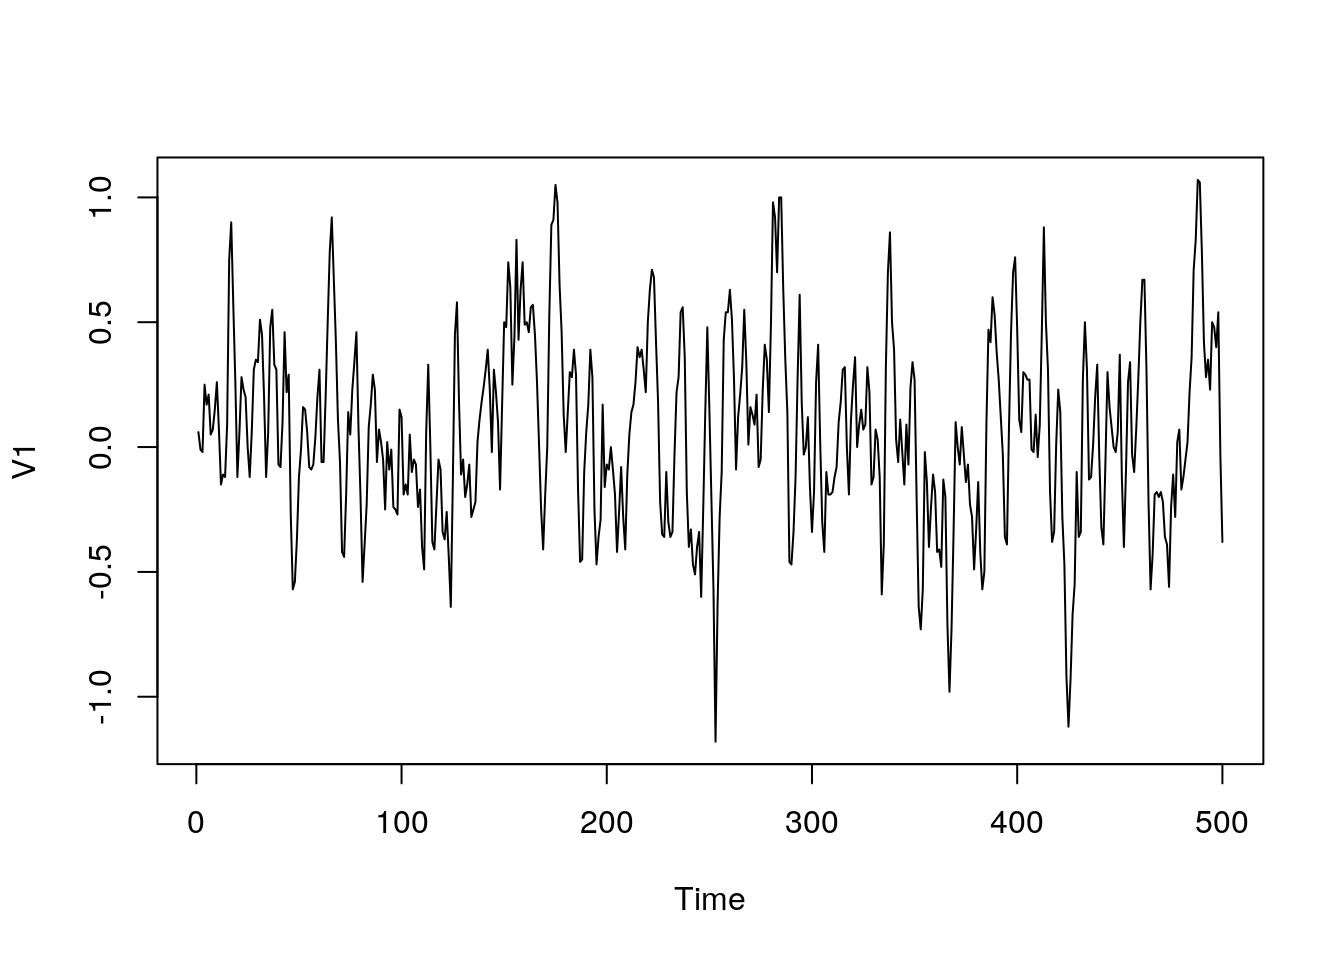
\includegraphics{Ex3_TImeSeries_files/figure-latex/unnamed-chunk-2-1.pdf}

\begin{Shaded}
\begin{Highlighting}[]
\KeywordTok{acf}\NormalTok{(dataseries) }\CommentTok{# Autocorrelation function}
\end{Highlighting}
\end{Shaded}

\includegraphics{Ex3_TImeSeries_files/figure-latex/unnamed-chunk-2-2.pdf}

\begin{Shaded}
\begin{Highlighting}[]
\KeywordTok{Pacf}\NormalTok{(dataseries) }\CommentTok{# Partial ACF}
\end{Highlighting}
\end{Shaded}

\includegraphics{Ex3_TImeSeries_files/figure-latex/unnamed-chunk-2-3.pdf}

\paragraph{Check for stationarity}\label{check-for-stationarity}

\begin{Shaded}
\begin{Highlighting}[]
 \CommentTok{#Check stationarity}
\KeywordTok{adf.test}\NormalTok{(dataseries) }\CommentTok{# Augmented Dickey-Fuller test}
\end{Highlighting}
\end{Shaded}

\begin{verbatim}
## Warning in adf.test(dataseries): p-value smaller than printed p-value
\end{verbatim}

\begin{verbatim}
## 
##  Augmented Dickey-Fuller Test
## 
## data:  dataseries
## Dickey-Fuller = -5.7437, Lag order = 7, p-value = 0.01
## alternative hypothesis: stationary
\end{verbatim}

\paragraph{Model fit}\label{model-fit}

\begin{Shaded}
\begin{Highlighting}[]
\CommentTok{# Estimate ARMA model coefficients using maximum likelihood}
\NormalTok{arimaFit <-}\StringTok{ }\KeywordTok{arima}\NormalTok{(dataseries, }\DataTypeTok{order =} \KeywordTok{c}\NormalTok{(}\DecValTok{2}\NormalTok{,}\DecValTok{0}\NormalTok{,}\DecValTok{1}\NormalTok{), }\DataTypeTok{method =} \StringTok{"ML"}\NormalTok{)}
\NormalTok{arimaFit}
\end{Highlighting}
\end{Shaded}

\begin{verbatim}
## 
## Call:
## arima(x = dataseries, order = c(2, 0, 1), method = "ML")
## 
## Coefficients:
##         ar1      ar2     ma1  intercept
##       0.929  -0.2651  0.2339     0.0615
## s.e.  0.096   0.0829  0.0968     0.0337
## 
## sigma^2 estimated as 0.0424:  log likelihood = 79.96,  aic = -149.92
\end{verbatim}

\begin{Shaded}
\begin{Highlighting}[]
\NormalTok{arimaFit}\OperatorTok{$}\NormalTok{sigma2}
\end{Highlighting}
\end{Shaded}

\begin{verbatim}
## [1] 0.04240467
\end{verbatim}

\begin{Shaded}
\begin{Highlighting}[]
\NormalTok{res_scaled <-}\StringTok{ }\NormalTok{arimaFit}\OperatorTok{$}\NormalTok{residuals}\OperatorTok{/}\KeywordTok{sqrt}\NormalTok{(arimaFit}\OperatorTok{$}\NormalTok{sigma2)}
\KeywordTok{plot}\NormalTok{(res_scaled)}
\end{Highlighting}
\end{Shaded}

\includegraphics{Ex3_TImeSeries_files/figure-latex/unnamed-chunk-4-1.pdf}

\begin{Shaded}
\begin{Highlighting}[]
\KeywordTok{hist}\NormalTok{(res_scaled)}
\end{Highlighting}
\end{Shaded}

\includegraphics{Ex3_TImeSeries_files/figure-latex/unnamed-chunk-4-2.pdf}

\paragraph{Analysis of the residuals}\label{analysis-of-the-residuals}

\begin{Shaded}
\begin{Highlighting}[]
\KeywordTok{acf}\NormalTok{(res_scaled) }\CommentTok{# To find order of MA(q) (lags)}
\end{Highlighting}
\end{Shaded}

\includegraphics{Ex3_TImeSeries_files/figure-latex/unnamed-chunk-5-1.pdf}

\begin{Shaded}
\begin{Highlighting}[]
\KeywordTok{pacf}\NormalTok{(res_scaled) }\CommentTok{# To find order of AR(p)}
\end{Highlighting}
\end{Shaded}

\includegraphics{Ex3_TImeSeries_files/figure-latex/unnamed-chunk-5-2.pdf}

\begin{Shaded}
\begin{Highlighting}[]
\KeywordTok{acf}\NormalTok{(dataseries)}
\end{Highlighting}
\end{Shaded}

\includegraphics{Ex3_TImeSeries_files/figure-latex/unnamed-chunk-5-3.pdf}

\begin{Shaded}
\begin{Highlighting}[]
\KeywordTok{pacf}\NormalTok{(dataseries)}
\end{Highlighting}
\end{Shaded}

\includegraphics{Ex3_TImeSeries_files/figure-latex/unnamed-chunk-5-4.pdf}

\begin{Shaded}
\begin{Highlighting}[]
\KeywordTok{vcov}\NormalTok{(arimaFit)}
\end{Highlighting}
\end{Shaded}

\begin{verbatim}
##                     ar1           ar2           ma1     intercept
## ar1        9.214698e-03 -7.437405e-03 -8.300512e-03 -3.400948e-07
## ar2       -7.437405e-03  6.869198e-03  6.850628e-03 -6.182259e-06
## ma1       -8.300512e-03  6.850628e-03  9.365246e-03 -2.403629e-07
## intercept -3.400948e-07 -6.182259e-06 -2.403629e-07  1.136831e-03
\end{verbatim}

\paragraph{Prediction for sample
values}\label{prediction-for-sample-values}

\begin{Shaded}
\begin{Highlighting}[]
\CommentTok{# QQplots}
\KeywordTok{qqnorm}\NormalTok{(res_scaled, }\DataTypeTok{main =} \StringTok{"Q-Q Plot: ARMA model"}\NormalTok{); }\KeywordTok{qqline}\NormalTok{(res_scaled) }\CommentTok{#Axis?}
\end{Highlighting}
\end{Shaded}

\includegraphics{Ex3_TImeSeries_files/figure-latex/unnamed-chunk-6-1.pdf}

\begin{Shaded}
\begin{Highlighting}[]
\CommentTok{# Predicted values of the model for the last 100 samples of the dataseries}
\NormalTok{Xhat <-}\StringTok{ }\KeywordTok{list}\NormalTok{()}
\NormalTok{phi1 <-}\StringTok{ }\NormalTok{arimaFit}\OperatorTok{$}\NormalTok{coef[}\DecValTok{1}\NormalTok{]; phi2 <-}\StringTok{ }\NormalTok{arimaFit}\OperatorTok{$}\NormalTok{coef[}\DecValTok{2}\NormalTok{]; theta1 <-}\StringTok{ }\NormalTok{arimaFit}\OperatorTok{$}\NormalTok{coef[}\DecValTok{3}\NormalTok{]; res <-}\StringTok{ }\NormalTok{arimaFit}\OperatorTok{$}\NormalTok{residuals}
\ControlFlowTok{for}\NormalTok{ (t }\ControlFlowTok{in} \DecValTok{3}\OperatorTok{:}\DecValTok{500}\NormalTok{)\{}
\NormalTok{  Xhat[t] =}\StringTok{ }\NormalTok{phi1}\OperatorTok{*}\NormalTok{dataseries[t}\OperatorTok{-}\DecValTok{1}\NormalTok{] }\OperatorTok{+}\StringTok{ }\NormalTok{phi2}\OperatorTok{*}\NormalTok{dataseries[t}\OperatorTok{-}\DecValTok{2}\NormalTok{] }\OperatorTok{+}\StringTok{ }\NormalTok{theta1}\OperatorTok{*}\NormalTok{res[t}\OperatorTok{-}\DecValTok{1}\NormalTok{] }\OperatorTok{+}\StringTok{ }\NormalTok{res[t]}
\NormalTok{\}}
\KeywordTok{plot}\NormalTok{(}\DecValTok{401}\OperatorTok{:}\DecValTok{500}\NormalTok{, dataseries[}\DecValTok{401}\OperatorTok{:}\DecValTok{500}\NormalTok{], }\StringTok{"l"}\NormalTok{)}
\KeywordTok{lines}\NormalTok{(}\DecValTok{401}\OperatorTok{:}\DecValTok{500}\NormalTok{, Xhat[}\DecValTok{401}\OperatorTok{:}\DecValTok{500}\NormalTok{], }\DataTypeTok{col =} \StringTok{"red"}\NormalTok{)}
\end{Highlighting}
\end{Shaded}

\includegraphics{Ex3_TImeSeries_files/figure-latex/unnamed-chunk-6-2.pdf}

\begin{Shaded}
\begin{Highlighting}[]
\CommentTok{# Add title, xlab and ylab}


\CommentTok{# Forecast}
\NormalTok{##################################################################}
\NormalTok{fcast =}\StringTok{ }\KeywordTok{forecast}\NormalTok{(arimaFit, }\DataTypeTok{h=}\DecValTok{20}\NormalTok{)}
\NormalTok{pred <-}\StringTok{ }\KeywordTok{predict}\NormalTok{(arimaFit, }\DataTypeTok{n.ahead =} \DecValTok{20}\NormalTok{, }\DataTypeTok{se.fit =} \OtherTok{TRUE}\NormalTok{)}
\KeywordTok{plot}\NormalTok{(fcast)}
\end{Highlighting}
\end{Shaded}

\includegraphics{Ex3_TImeSeries_files/figure-latex/unnamed-chunk-6-3.pdf}

\paragraph{AICc}\label{aicc}

\begin{Shaded}
\begin{Highlighting}[]
\CommentTok{# AIC}
\NormalTok{arimaFit}\OperatorTok{$}\NormalTok{aic}
\end{Highlighting}
\end{Shaded}

\begin{verbatim}
## [1] -149.9161
\end{verbatim}

\begin{Shaded}
\begin{Highlighting}[]
\CommentTok{# Plots of AIC}
\CommentTok{# Which order p,q is best, compare AIC}
\NormalTok{frame <-}\StringTok{ }\KeywordTok{data.frame}\NormalTok{(}\DataTypeTok{p =} \DecValTok{0}\NormalTok{, }\DataTypeTok{q =} \DecValTok{0}\NormalTok{, }\DataTypeTok{aic =} \DecValTok{0}\NormalTok{)}
\ControlFlowTok{for}\NormalTok{(p }\ControlFlowTok{in} \DecValTok{1}\OperatorTok{:}\DecValTok{5}\NormalTok{)\{}
  \ControlFlowTok{for}\NormalTok{(q }\ControlFlowTok{in} \DecValTok{1}\OperatorTok{:}\DecValTok{5}\NormalTok{)\{}
\NormalTok{    fit <-}\StringTok{ }\KeywordTok{arima}\NormalTok{(dataseries, }\DataTypeTok{order =} \KeywordTok{c}\NormalTok{(p,}\DecValTok{0}\NormalTok{,q), }\DataTypeTok{method =} \StringTok{"ML"}\NormalTok{)}
\NormalTok{    frame <-}\StringTok{ }\KeywordTok{rbind}\NormalTok{(frame, }\KeywordTok{c}\NormalTok{(p,q,fit}\OperatorTok{$}\NormalTok{aic))}
\NormalTok{  \}}
\NormalTok{\}}
\end{Highlighting}
\end{Shaded}

\begin{verbatim}
## Warning in arima(dataseries, order = c(p, 0, q), method = "ML"): possible
## convergence problem: optim gave code = 1

## Warning in arima(dataseries, order = c(p, 0, q), method = "ML"): possible
## convergence problem: optim gave code = 1

## Warning in arima(dataseries, order = c(p, 0, q), method = "ML"): possible
## convergence problem: optim gave code = 1

## Warning in arima(dataseries, order = c(p, 0, q), method = "ML"): possible
## convergence problem: optim gave code = 1
\end{verbatim}

\begin{Shaded}
\begin{Highlighting}[]
\NormalTok{frame <-}\StringTok{ }\NormalTok{frame[}\OperatorTok{-}\DecValTok{1}\NormalTok{,]}
\KeywordTok{ggplot}\NormalTok{(frame, }\KeywordTok{aes}\NormalTok{(p,q)) }\OperatorTok{+}\StringTok{ }\KeywordTok{geom_raster}\NormalTok{(}\KeywordTok{aes}\NormalTok{(}\DataTypeTok{fill =}\NormalTok{ aic)) }\CommentTok{#+ scale_fill_gradientn(colours=c("#0000FFFF","#FFFFFFFF","#FF0000FF")) # Alternative color gradient}
\end{Highlighting}
\end{Shaded}

\includegraphics{Ex3_TImeSeries_files/figure-latex/unnamed-chunk-7-1.pdf}

\subsubsection{Discussion}\label{discussion}

\begin{itemize}
\item
  Comments on prelim plots: time series, ACF, PACF
\item
  Comments on estimated paramateres and uncertainties in particular
\item
  Comments on fit/prediction of the chosen ARMA model
\item
  Finally, comment on the diagnostics, AICC
\end{itemize}

\subsubsection{Conclusion}\label{conclusion}

\subsubsection{Appendix, References}\label{appendix-references}


\end{document}
